\documentclass[a4paper,11pt]{article}
\usepackage[left=2.5cm, right=2.5cm, top=1.5cm, bottom=1.5cm]{geometry}
\usepackage{graphicx}
\usepackage{amssymb}
\usepackage{amsmath}
\usepackage{hyperref}
\usepackage{cleveref}
\usepackage{float}
\usepackage[table,xcdraw]{xcolor}
\usepackage{subcaption}

\hypersetup{ %color attributes of citation, link, etc.
    colorlinks=true,
    linkcolor=blue,
    filecolor=gray,
    urlcolor=blue,
    citecolor=blue,
}

\setlength{\parindent}{0pt}

\newcommand{\matlab}{\textsc{Matlab}} %very important and totally necessary addition
\newcommand{\parallelsum}{\mathbin{\!/\mkern-5mu/\!}}

\newcommand\Item[1][]{%
  \ifx\relax#1\relax  \item \else \item[#1] \fi
  \abovedisplayskip=0pt\abovedisplayshortskip=0pt~\vspace*{-\baselineskip}}

%'codify' text for snippets
\usepackage{xcolor}
\definecolor{codegray}{gray}{1}
\newcommand{\code}[1]{\colorbox{codegray}{\texttt{#1}}}


\graphicspath{ {./images/} }
           
\begin{document}
\title{\LARGE{\textbf{ECEN405 D-Class Amplifier}}\\ \large{\textit{`What a buck converter would say if it could talk'}}}
\author{Niels Clayton : 300437590\\
\textbf{Team Members:} Daniel Eisen \& Nickolai Wolfe}
\date{}
\maketitle

\begin{center}
    \vspace{-20pt}
    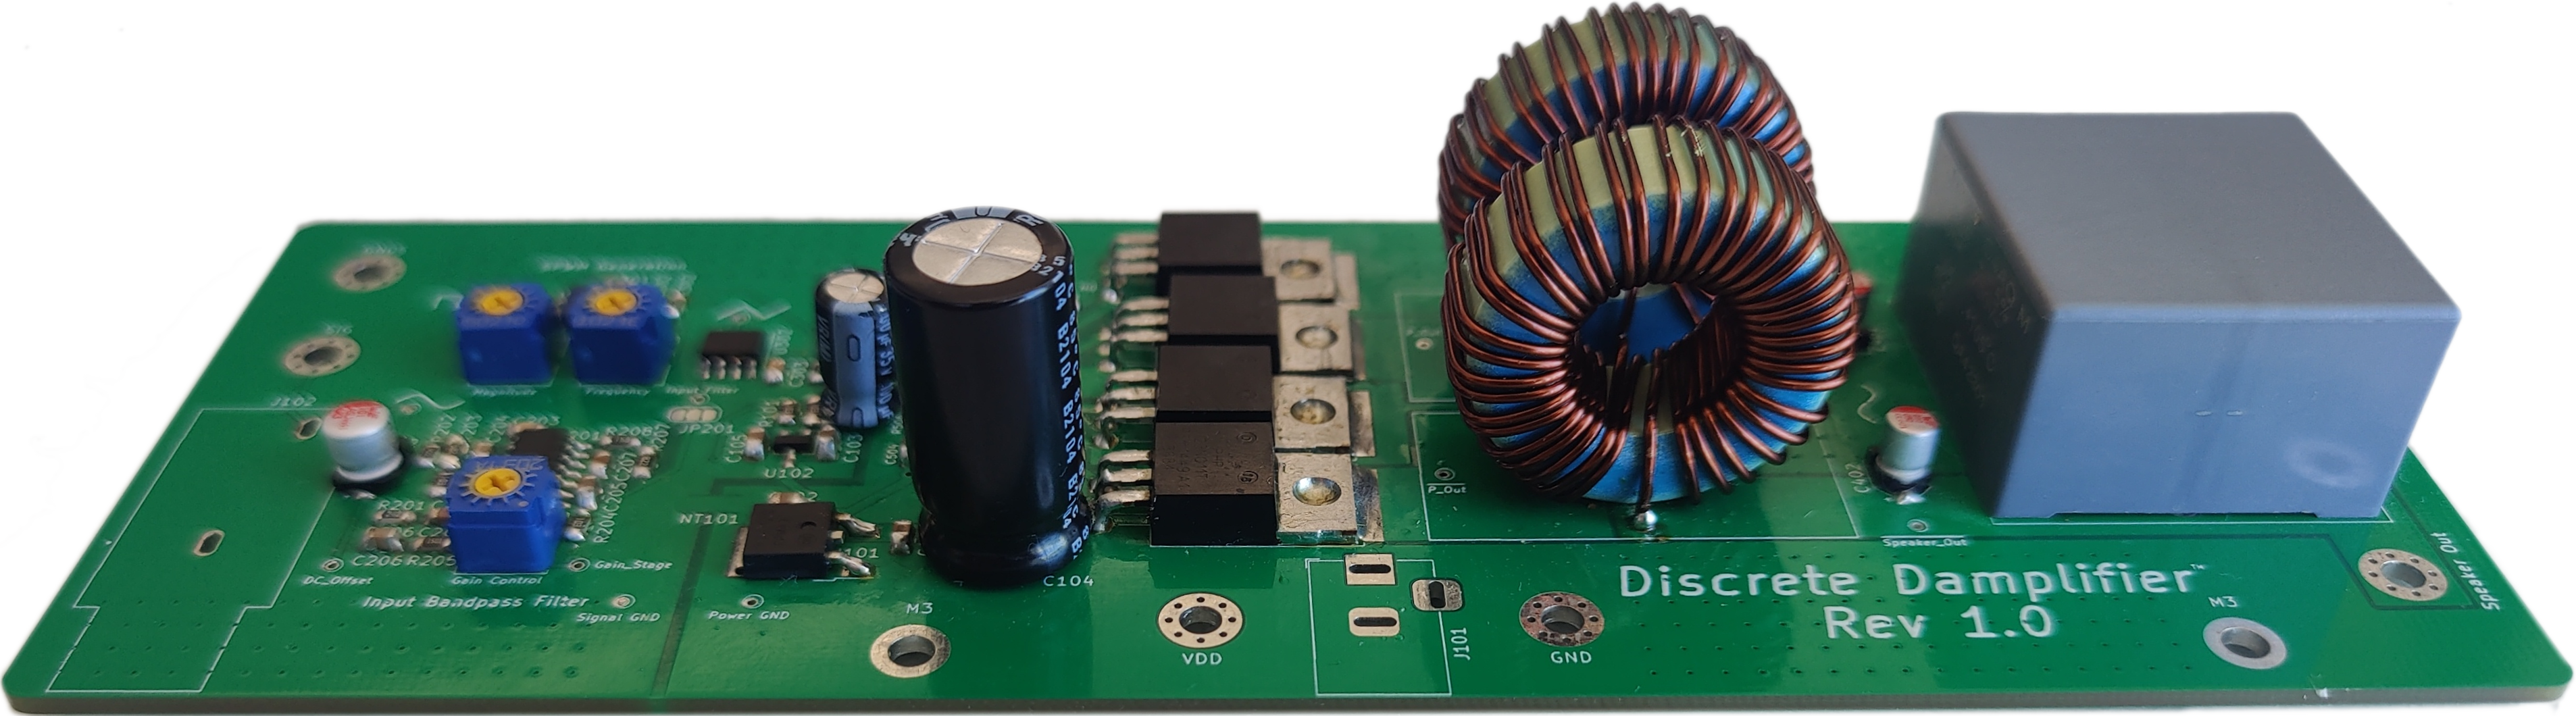
\includegraphics[width=0.9\textwidth]{design.png}
\end{center}

\section{Introduction}\label{S:intro}

Audio amplifiers facilitate the driving of high power speakers from small signal audio outputs. Common amplifier types for high fidelity audio are the class A and AB amplifier. These amplifiers provide high power outputs and very little distortion, with the limitation of low power efficiency. The efficiency losses in these topologies are due to the continuous operation of their amplifying elements (usually BJT's) within their saturation region, generating large continuous losses in the form of heat.

In contrast, the class D amplifier is a high efficiency power amplifier. These high efficiencies are achieved through the use of switching elements as amplifiers, allowing for no continuous power loss within the design. This topology can provide efficiencies of up to 90-95\%, with the limitation of greatly increased design complexity.\\

The purpose of this reports is to discuss the design and implementation of a class D amplifier for use in driving a sub-woofer speaker to given specifications outlined in \Cref{S:specs}. This project was completed in a group of three, where I have taken responsibility for the audio sampling and sinusoidal pulse width modulation (SPWM) generation designs. We have all contributed equally to the final PCB and schematic designs. 

\subsection{Specifications}\label{S:specs}

\begin{itemize}
    \item Supply 80W of power into a 4$\Omega$ load $\rightarrow P_{out} = 80W$ for $R_L = 4\Omega$.
    \item Have a 10Hz to 200Hz operating bandwidth.
    \item Have an input sensitivity of 1V for maximum output.
    \item Cost a maximum of \$50 per unit.
\end{itemize}

\section{Design}\label{S:design}

The operation of a class D amplifier can be broken down into discrete sections that are outlined in \Cref{F:block}. From this figure we see that the first section is the input audio signal filter, which acts to remove unwanted signal components from the input audio before amplification. In the next stage this filtered audio is sampled at high frequency using a triangle wave and a comparator to produce a high frequency SPWM carrier signal. Finally, this SPWM signal is then amplified to a high power output with a MOSFET before being low pass filtered again to remove the SPWM carrier frequency.

\begin{figure}[h!]
    \centering
    \frame{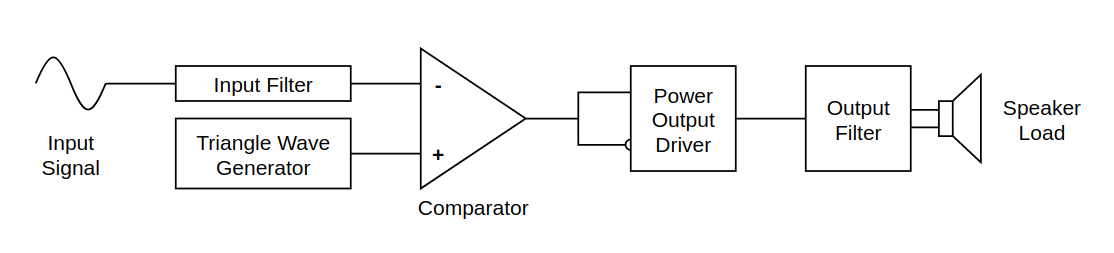
\includegraphics[width=0.8\textwidth]{block_diagram.png}}
    \caption{D-Class amplifier high level block diagram}
    \label{F:block}
\end{figure}

\subsection{High Level Design Decisions}

The high level design of this class D amplifier consisted of two decision, the selection of amplifier topology, and the selection of the input supply voltage level and supplies.\\

The exists two topologies for the design of class D amplifiers, half-bridge and full-bridge. The differentiating feature of these topologies is the configuration of their switching elements, with full-bridge requiring four MOSFETS and two gate drivers, while half-bridge requires two MOSFETS and a single gate driver. This has the affect of requiring the half-bridge topology to drive both the positive and negative portions of the output through a single MOSFET bridge, therefore requiring double the input voltage to achieve the same output power as the full-bridge topology. The half-bridge topology can also cause large fluctuations in the supply rail for the amplification, and therefore will often be accompanied by a feedback controller to account for these supply changes. Because of the design complications of the half-bridge topology, our design will implement the full-bridge class D amplifier.\\

For the selection of the designs power supply, it was decided that a single supply rail should be provided to the amplifier, with all other required voltage levels being generated internally. This was selected to provide a more cohesive and easy to operate final design. Based on this design, the required input voltage ($V_{DD}$) to achieve the specified output power of 80W has been calculated in the following equation to be 26V. This is then stepped down to both 12V and 5V internally though thee use of linear regulators. A 1000$\mu$F reservoir capacitor was also selected to reduce the strain on the input power supply from the high frequency high power switching elements.

$$ V_{DD} = \sqrt{2\cdot R_L \cdot P_{out}} = \sqrt{2\cdot 4 \cdot 80} = 25.29 \approx 26$$

In \Cref{F:design_schemtaic} we can see the finalised high-level schematic design of the amplifier. In this schematic the input supply stages can be found, as well as the high level design of the amplifier as discussed in \Cref{S:design}. 

\begin{figure}[h!]
    \centering
    \frame{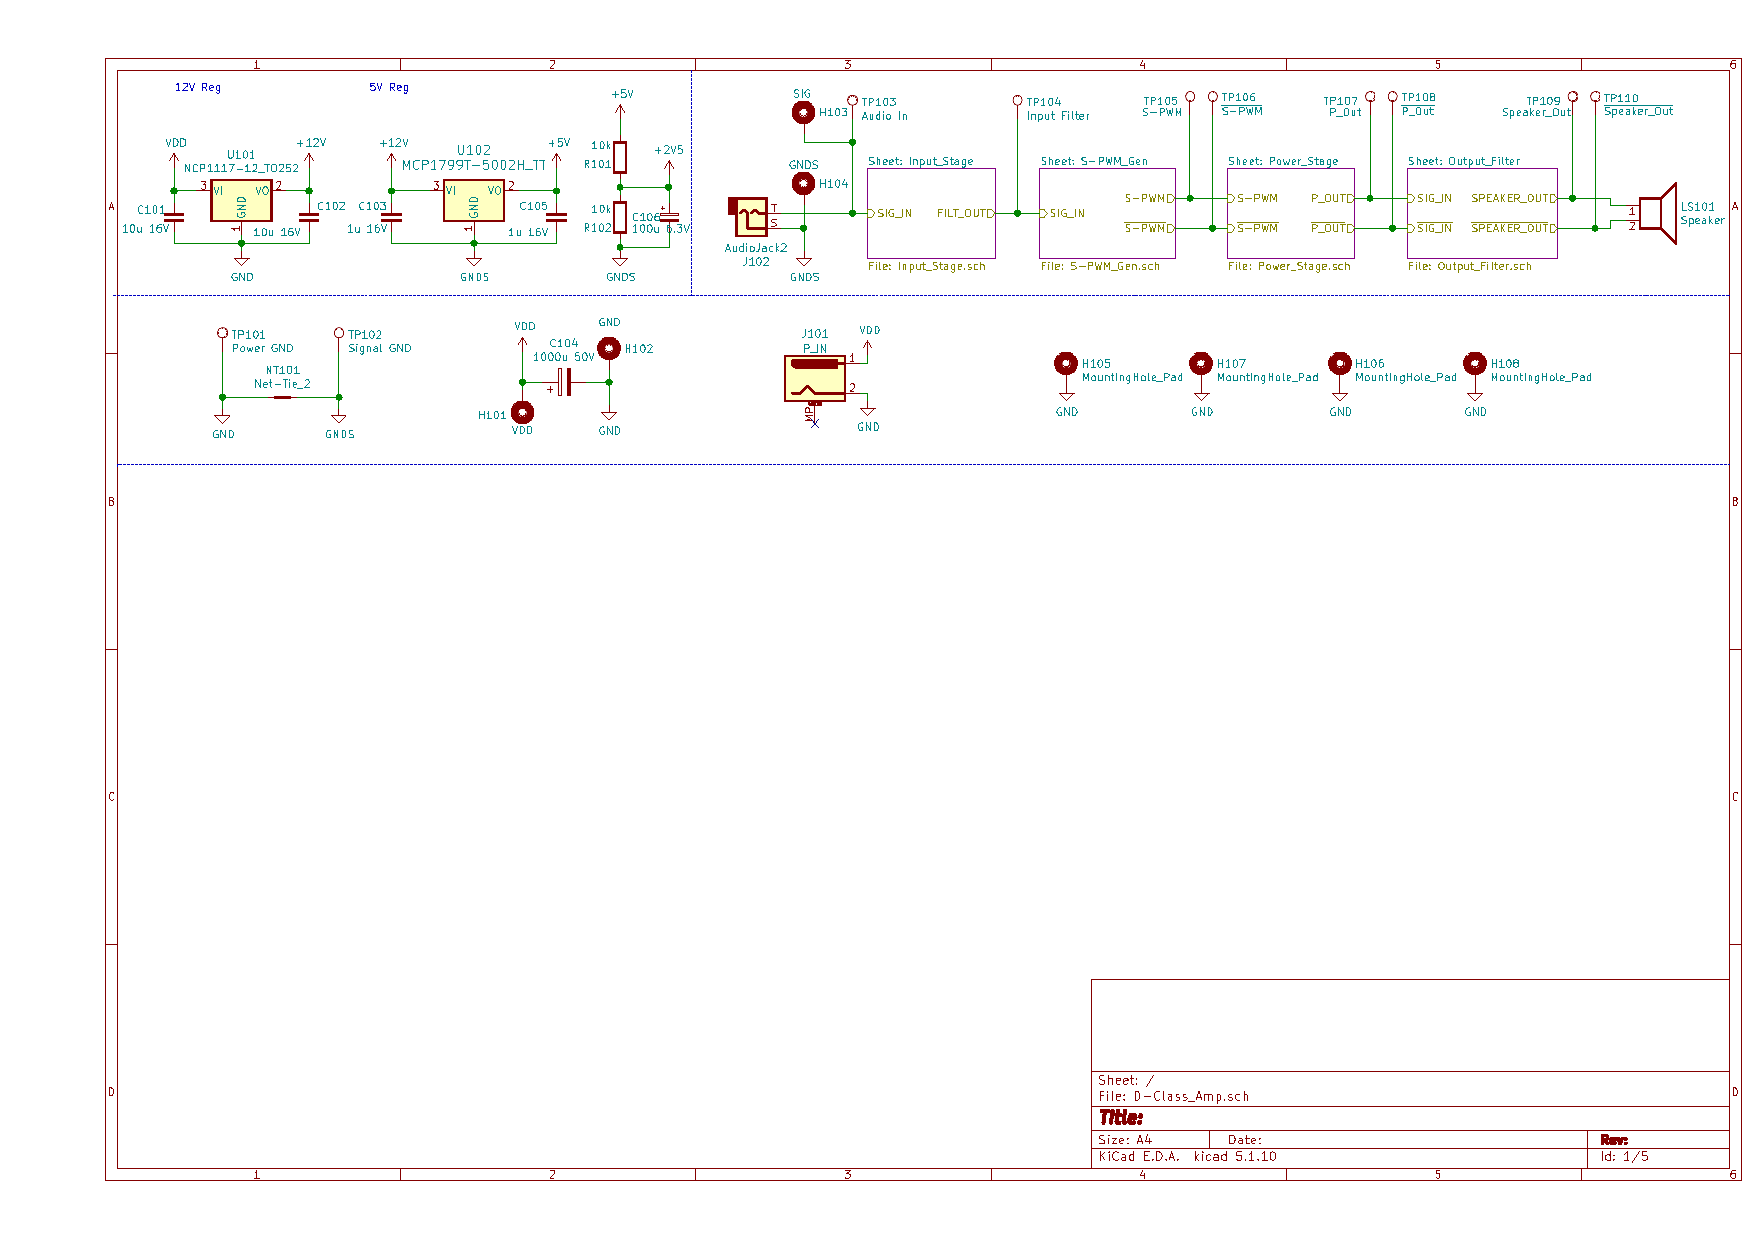
\includegraphics[page=1, trim={18mm 132mm 2mm 10mm},clip,width=0.85\textwidth]{pcb/schematic.pdf}}
    \caption{High level design schematic}
    \label{F:design_schemtaic}
\end{figure}

\subsection{Input Filter}

The design of the input filter was required to provide a signal passband of 10Hz to 200Hz, and function correctly for input signals of up to 1V amplitude, 2V$_{pk-pk}$ as specified in \Cref{S:specs}. The design of this section was undertaken by Nickolai Wolfe, and the finalised schematic of this can be seen in \Cref{F:input_filter_design}.


\begin{figure}[h!]
    \centering
    \frame{\includegraphics[page=2, trim={25mm 70mm 90mm 60mm},clip,width=0.85\textwidth]{pcb/schematic.pdf}}
    \caption{Input filtering schematic}
    \label{F:input_filter_design}
\end{figure}

This design consists of a forth order low pass active Butterworth filter with a cut-off frequency of 300Hz, and a second order high pass active Butterworth filter with a cut-off frequency of 10Hz. This provides 40dB per decade gain roll-off for inputs frequencies below 10Hz, as well as a 80dB per decade gain roll-off for inputs frequencies above 300Hz. It should also be noted that the placement of the low pass corner frequency at 300Hz ensures that there is a constant 0dB gain across the full specified bandwidth of the amplifier. \\

The output signal of the input filter has a DC bias of 2.5V imposed on it. This has been implemented to `mid-rail' the opamps utilised within this design, allowing them to function correctly from a single 5V DC supply.

This input stage also provides an amplifier gain stage to allow for tuning of the filter output amplitude to vary between 1V$_{pk-pk}$ and 3V$_{pk-pk}$.   

\subsection{Audio Sampling \& SPWM}

The audio sampling and SPWM generation stage requires the generation of a high quality high frequency triangle waveform. This waveform is compared to the input audio signal with a comparator, facilitating the production of an SPWM carrier signal where the PWM duty cycle encodes the input signal voltage at that given sample.\\

The design requirements for this section have been selected to ensure that all requirements outlined in \Cref{S:specs} are met, and such that interfacing with both the input filter and the power amplification stage is simple.  

With these requirements, the following set of specifications for this design were devised. 
\begin{itemize}
    \item  The sampler must produce a triangle wave sampling signal with a switching frequency of at least a decade greater than the highest sampled frequency (200Hz).
    \item THe triangle wave must be imposed on the 2.5V DC offset.
    \item The sampler must providing the full range of operation for inputs between 1V$_{pk-pk}$ and 3V$_{pk-pk}$ from the input filter.
    \item The SPWM output must be between 0V and 5V to correctly interface with the selected gate drivers.
    \item The SPWM output must provide both an inverted and non-inverted output to drive each half bridge.
\end{itemize}

The sampling triangle wave was generated using an unstable positive feedback opamp oscillator. This circuit design consists of two opamp stages, the first uses positive feedback to cause an opamp to oscillate between it's voltage rails and create a square wave, the second integrates this square wave to produce triangle wave. An overview of this circuit can be seen in \Cref{F:spice_circuit}.

Due to this designs reliance on the selected opamps specifications, it becomes difficult to design the exact frequency of the circuits output, however the following equation provides a rough estimate of the output frequency for a given selection of values. 

\begin{align*}
    f &= \frac{R_2}{4(R_1 \cdot R_3 \cdot C_1)} 
\end{align*}

Using this equation, components were calculated that would provide an output triangle wave with a frequency of 30kHz, as this is above the minimum sampling frequency specification of 20kHz. 

With these initial components selected, the design was tested within the circuit simulation software LTSpice. A wide assortment of opamp spice models were sourced for the design simulations, with varying slewrates and gain bandwidth products (GBP). Simulations were run across this range of opamps for frequencies between 30kHz and 100kHz, allowing for the comparison and selection of the lowest cost opamp that would be capable of providing the designed switching frequency. 

This simulation also allowed for the selection of the triangle wave peak to peak voltage though testing various values for $R_3$. 


\begin{figure}[h!]
    \centering
    \frame{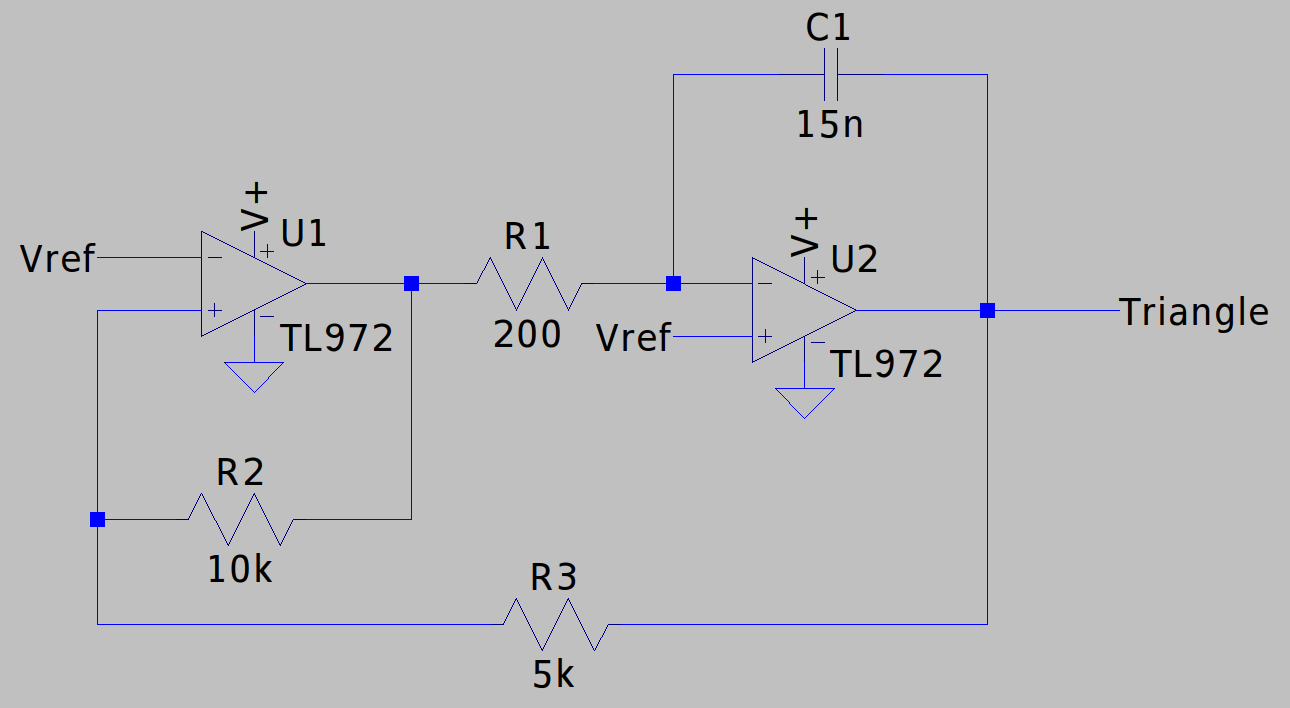
\includegraphics[width=0.5\textwidth]{spwm/circuit.png}}
    \caption{Triangle waveform generation circuit}
    \label{F:spice_circuit}
\end{figure}

 The final designed circuit can be seen in \Cref{F:sampling_schematic}. This circuit utilised the TL972 dual opamp to provide a 2V$_{pk-pk}$ 32kHz triangle wave that would also be capable of operating at frequencies of up to 100kHz. 
 
 This dual opamp package is capable of implementing the full design. It has also been shown from simulations in \Cref{F:triangle} show that this opamp is capable of producing a triangle wave with switching frequency and magnitude that meet the given requirements.

 In \Cref{F:sampling} we can see a simulation of a 2V$_{pk-pk}$ input signal within the envelop of the designed triangle. From this we confirm the design is capable of sampling the full input signal range without distortion or clipping. We can also see from both of these figures that the generated triangle wave is imposed on a 2.5V DC offset as specified. 

\begin{figure}[h!]
    \centering
    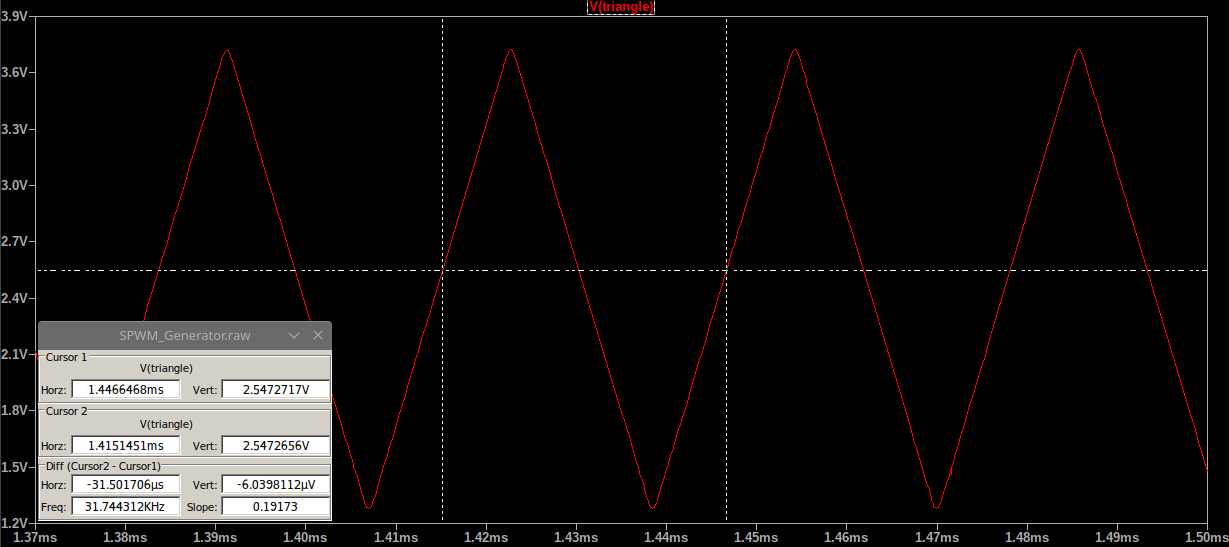
\includegraphics[width=0.7\textwidth]{simulation/triangle_wave.png}
    \caption{Simulation of the generated 32kHz triangle waveform}
    \label{F:triangle}
\end{figure}

\begin{figure}[h!]
    \centering
    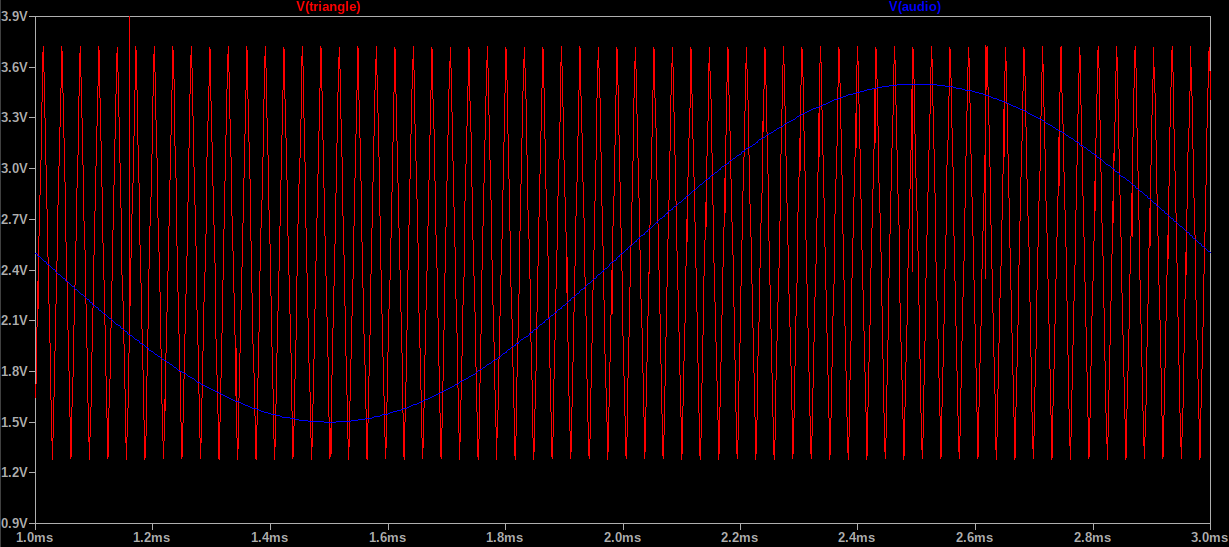
\includegraphics[width=0.7\textwidth]{simulation/sampling.png}
    \caption{Simulation of a 1V peak to peak input signal sampling}
    \label{F:sampling}
\end{figure}

\begin{figure}[h!]
    \centering
    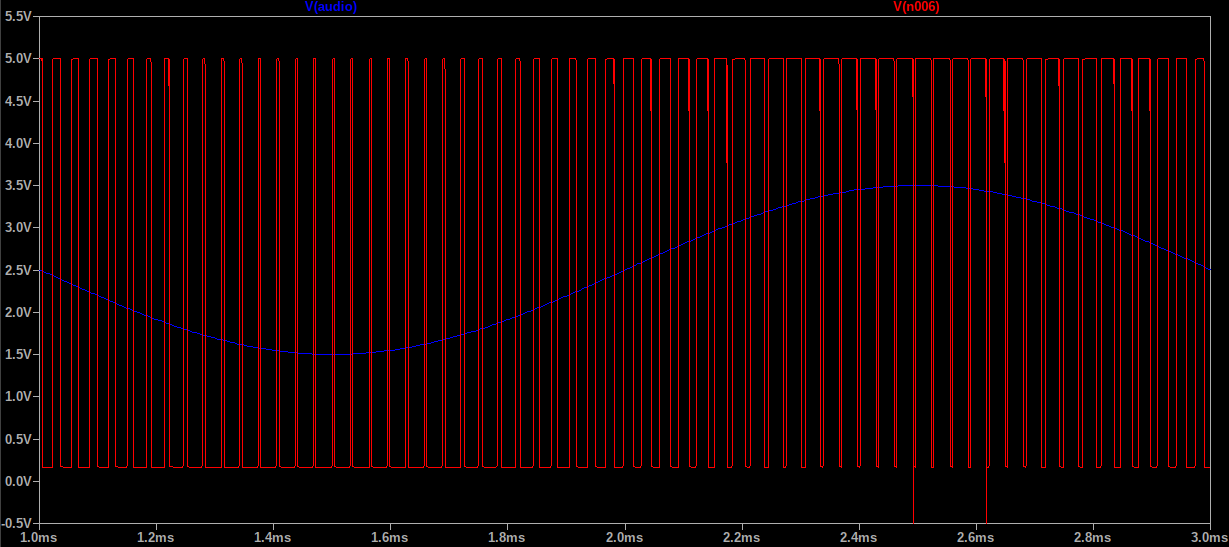
\includegraphics[width=0.7\textwidth]{simulation/spwm_out.png}
    \caption{Simulation of the SPWM comparator output}
    \label{F:SPWM}
\end{figure}

Next to design was the SPWM generation circuit. This circuit had the requirement of taking both the audio signal to be sampled, and the sampling triangle waveform, and comparing them to provide a 5V output. It was also required to provide both an inverted and non-inverted signal output.

To achieve this, a high speed open collector comparator should be used. By selecting an open collector comparator, the output voltage can be defined through the used of a simple voltage pullup resistor. The selected comparator was the LMV393 with a 1k$\Omega$ pullup resistor. To provide both an inverted and non-inverted output, a dual package comparator was selected, by switching the input terminals of one of the comparators, the signal will be inverted with respect to the other.\\

Simulations of this SPWM output signal can be found in \Cref{F:SPWM}, in which it can be seen that the output signal goes between 0V and 5V, and the duty cycle of the PWM varies depending on the current audio input.

\begin{figure}[h!]
    \centering
    \frame{\includegraphics[page=3, trim={35mm 133.5mm 30mm 15mm},clip,width=0.85\textwidth]{pcb/schematic.pdf}}
    \caption{Sampling triangle wave \& SPWM generation schematic}
    \label{F:sampling_schematic}
\end{figure}

The final design and schematic of this section can be seen in \Cref{F:sampling_schematic}. In this schematic it can be noted that in the triangle wave generator, resistors $R_1$ and $R_3$ have potentiometers in series. This provides the ability to externally tune both the triangle wave frequency between 30kHz and 100kHz, and the scaling between 1V$_{pk-pk}$ and 3V$_{pk-pk}$. 

This will allow for the selection of the highest performing switching frequency, as well as the tuning of the sampling to directly match the output of the input filter. 


\subsection{Power Stage \& Output Filter}

The design of the power stage and output filter was required to amplify the generated SPWM signals from the sampler to V$_{DD}$ using MOSFET bridges, and then low pass filter this output to remove the SPWM carrier frequency. The design of this section was undertaken by Daniel Eisen.\\

In \Cref{F:gate_driver} the finalised schematic for the MOSFETS and gate drivers can be seen. From this figure it can be seen that this design is split into two symmetrical half-bridge gate drivers, providing the full-bridge topology. This provides the ability to take inputs from both the inverted and non-inverted 5V SPWM signals generated by the sampling stage, and directly step them up to the supply voltage rail.

The gate drivers also provide bootstrapping for the operation of the high-side N-channel MOSFETS, and programmable dead-time.

\begin{figure}[h!]
    \centering
    \frame{\includegraphics[page=5, trim={85mm 149mm 5mm 12mm},clip,width=0.85\textwidth]{pcb/schematic.pdf}}
    \caption{Gate driver schematic}
    \label{F:gate_driver}
\end{figure}

In \Cref{F:output_filter} we can see the the finalised schematic of the output filter. This is a passive second order low pass filter with a cut-off frequency of 3kHz. This cut-off frequency will guarantee a minimum sampling frequency attenuation of 40dB, and has the possibility to provide greater attenuation at increased sampling frequencies.   

\begin{figure}[h!]
    \centering
    \frame{\includegraphics[page=4, trim={115mm 97mm 105mm 75mm},clip,width=0.6\textwidth]{pcb/schematic.pdf}}
    \caption{Output filter schematic}
    \label{F:output_filter}
\end{figure}

\section{Implementation}  

This section will discuss the implementation decision made on this project, as well as the issues faces when implementing this project. 

\subsection{PCB Design and Layout}

With the final design of the class D amplifier schematic complete, the implementation of the design in the form of a printed circuit board (PCB) began. In \Cref{F:PCB} we are able to see the final layouts of this designed PCB, including the traces, and both the top and bottom copper pour layers.\\

As the design of this PCB included both small signal processing at the audio input, and high frequency high power switching at the power output, it was very important to correctly isolate the analog and power ground planes. 

To achieve this, a net tie was used to separate the analog and power grounds, and provide a single connection location. This allows for the definition of the current return path of the analog section, ensuring that no high current switching can return underneath sensitive components. These separations can be clearly seen in \Cref{F:PCB_top} \& \Cref{F:PCB_bottom}\\

The PCB also features heavy via stitching between the top and bottom copper planes. This is done to both improve the thermal performance of the components, and to ensure there are no potential differences between these two planes. 

It can also be noted that all high current paths have been placed using copper pours, providing very low impedance paths.

\begin{figure}[h!]
    \centering
    \begin{subfigure}{0.8\textwidth}
        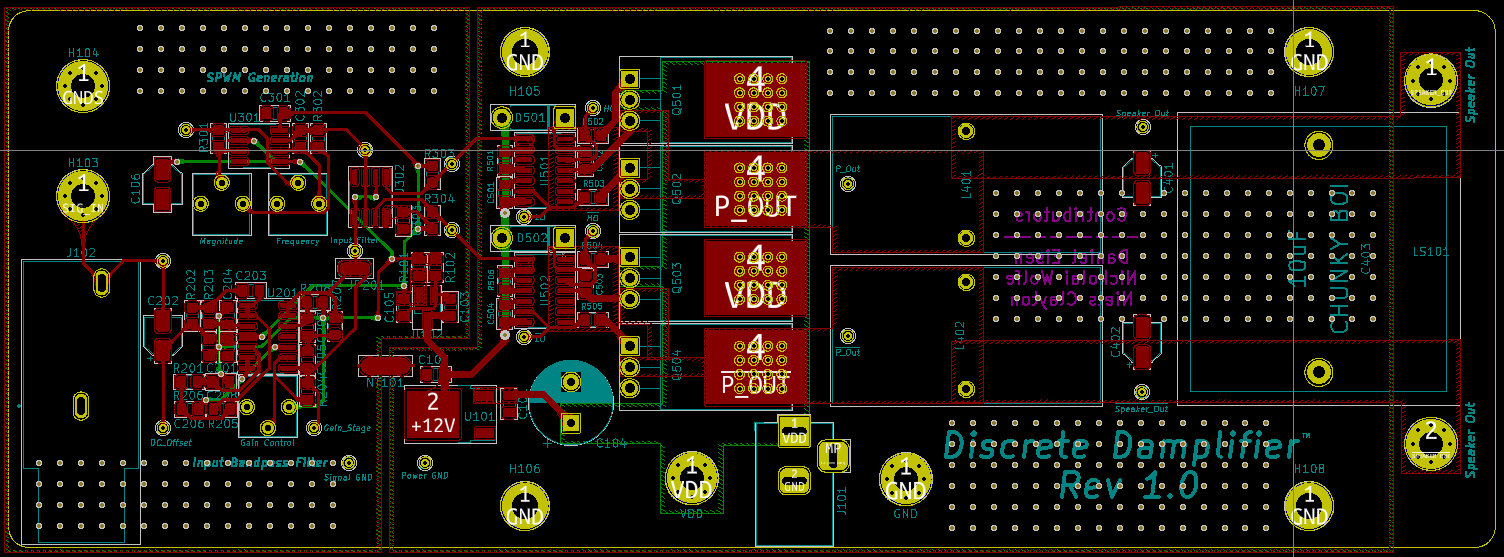
\includegraphics[width=\columnwidth]{pcb/traces.png}
        \subcaption{PCB Traces}
        \label{F:PCB_traces}
    \end{subfigure}
    \begin{subfigure}{0.8\textwidth}
        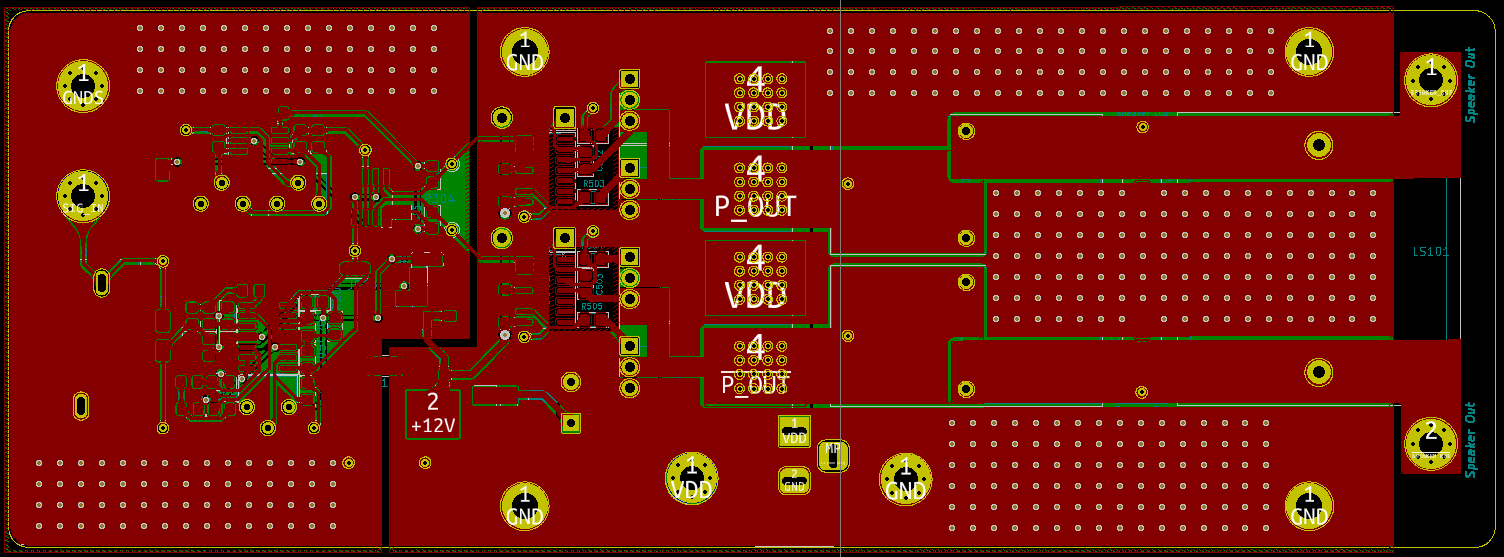
\includegraphics[width=\columnwidth]{pcb/top_layer.png}
        \subcaption{PCB top layer copper pours}
        \label{F:PCB_top}
    \end{subfigure}
    \begin{subfigure}{0.8\textwidth}
        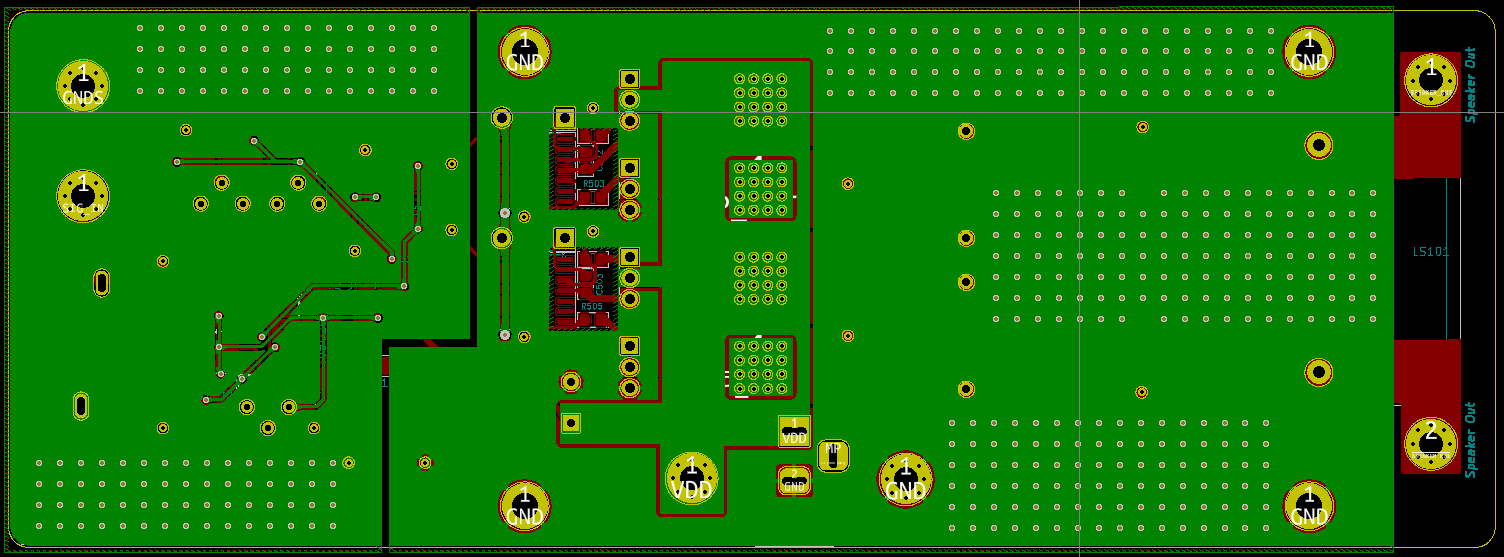
\includegraphics[width=\columnwidth]{pcb/bottom_layer.png}
        \subcaption{PCB bottom layer copper pours}
        \label{F:PCB_bottom}
    \end{subfigure}
    \caption{Design PCB layouts}
    \label{F:PCB}
\end{figure}

\subsection{Audio Sampling \& SPWM}

The initial implementation of the audio sampling triangle wave was unsuccessful. This can be attributed to errors in the manufacturer provided SPICE simulation models of the TL972 opamp, leading to the design being incapable of meeting it's designed requirements. This issue was quickly remedied however as the dual opamp utilised the common SOIC-8 SMD package, this allowed me to easily exchange the opamp for a higher bandwidth LMH6658 opamp. \\

After the replacement opamp was installed, testing was performed to verify the functionality of the audio sampling design. 

In \Cref{F:triangle_implemented} the output sampling triangle wave of the implemented circuit can be seen. From this scope image it can be verified that a switching frequency of 32kHz was achieved as designed. It should also be noted that through tuning of the implemented potentiometers it is capable to achieve switching frequencies well beyond 200kHz.

In \Cref{F:sampling_implemented} we can see the triangle waveform directly sampling a 100Hz 2V$_{pk-pk}$ input waveform, and in \Cref{F:envelope_implemented} we can see a larger time scale of this sampling. From these two figures we can confirm that the sampling envelop is able to fully sample inputs to the required specifications. It should also be noted that the triangle wave scaling potentiometer is functional, and it is possible to sample inputs ranging between 1V$_{pk-pk}$ and 3V$_{pk-pk}$ as designed.

\begin{figure}[h!]
    \centering
    \begin{subfigure}{0.52\textwidth}
        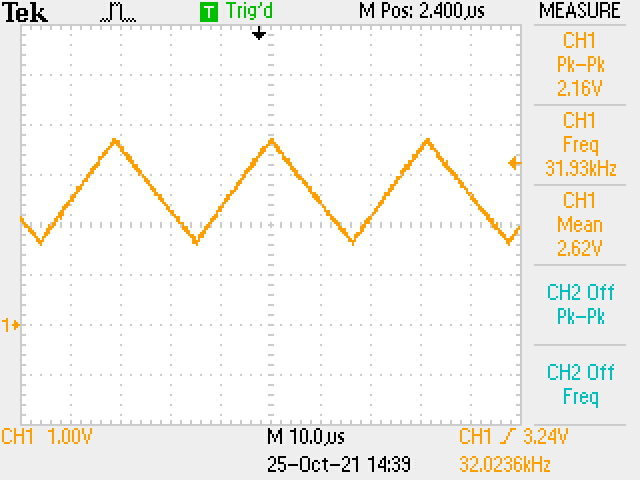
\includegraphics[width=0.85\columnwidth]{spwm/triangle_wave_32kHz.JPG}
        \subcaption{Generated sampling triangle wave}
        \label{F:triangle_implemented}
    \end{subfigure}
    \begin{subfigure}{0.49\textwidth}
        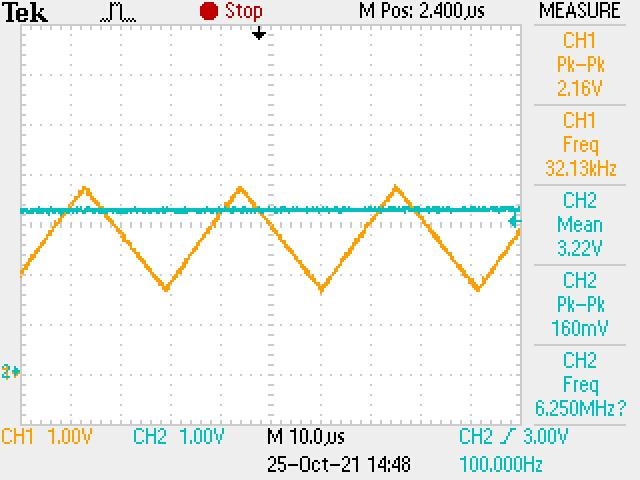
\includegraphics[width=0.85\columnwidth]{spwm/input_sampling_1.JPG}
        \subcaption{Triangle wave sampling input signal}
        \label{F:sampling_implemented}
    \end{subfigure}
    \begin{subfigure}{0.49\textwidth}
        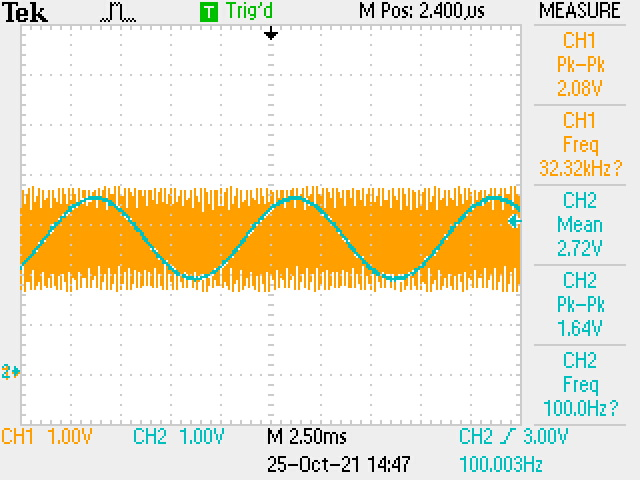
\includegraphics[width=0.85\columnwidth]{spwm/input_sampling_0.JPG}
        \subcaption{Triangle wave sampling envelop of input signal}
        \label{F:envelope_implemented}
    \end{subfigure}
    \caption{}
\end{figure}

Finally, we can confirm the operation of the comparators, and the functionality of the SPWM generation. In \Cref{F:SPWM_implemented} we see the comparator output when not input audio is supplied. As expected, this produces a 50\% duty cycle PWM output between 0V and 5V.

\begin{figure}[H]
    \centering
    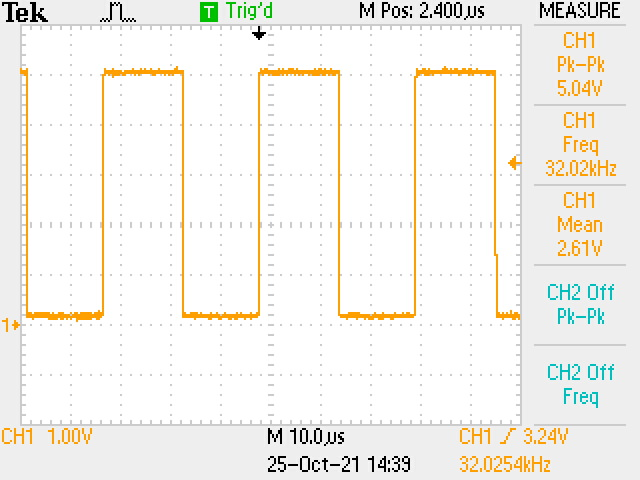
\includegraphics[width=0.4\textwidth]{spwm/spwm_no_input.JPG}
    \caption{Amplifier output bode plot}
    \vspace{-20pt}
    \label{F:SPWM_implemented}
\end{figure}


\section{Results}

After the successful implementation of the design, a selection of tests were performed to characterise the output of out amplifier, and confirm that we meet all the required specifications.\\

The first series of test performed were to simply observe the loaded output waveform from the amplifier and a range of frequencies. The outputs of this can be seen in \Cref{F:output_plotting}, in these figures we can visually inspect both the functionality of the input and output filters, as well as observe any distortion on the waveform. 

When looking at \Cref{F:out_1hz} we can clearly see that there is attenuation of the output caused by the high pass input filter, and we can observe in \Cref{F:out_10hz}, that at the 10Hz cut-in frequency this attenuation is mostly gone. Then from \Cref{F:out_100hz} \& \Cref{F:out_200hz} it can be observed that throughout the passband of the filters, there is no attenuation of the output signal, and finally in \Cref{F:out_500hz} \& \Cref{F:out_2khz} we can clearly see the 80dB per decade attenuation of the output.\\

It can also clearly be seen from these output waveforms that there is little to no noticeable output waveform distortion, and no visible switching from the SPWM carrier frequency.

\begin{figure}[H]
    \centering
    \begin{subfigure}{0.3\textwidth}
        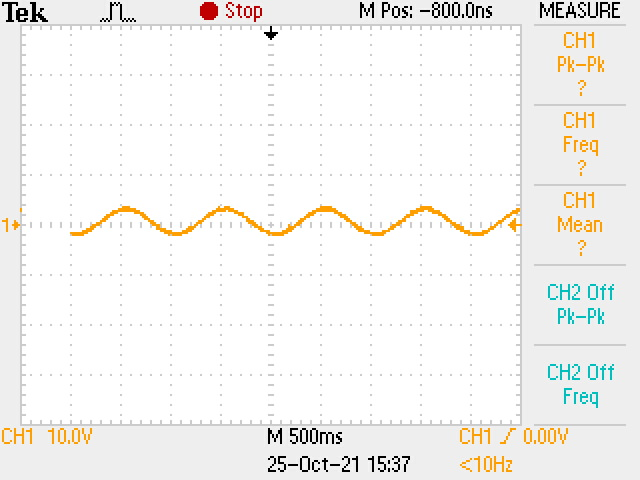
\includegraphics[width=\columnwidth]{power_output/filter_output_1Hz.JPG}
        \subcaption{1Hz}
        \label{F:out_1hz}
    \end{subfigure}
    \begin{subfigure}{0.3\textwidth}
        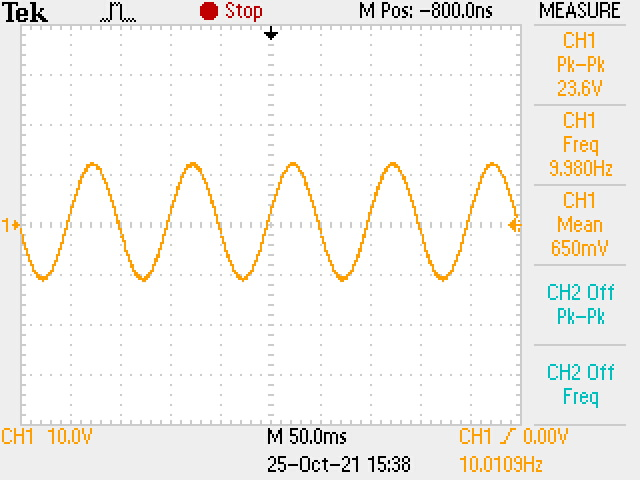
\includegraphics[width=\columnwidth]{power_output/filter_output_10Hz.JPG}
        \subcaption{10Hz}
        \label{F:out_10hz}
    \end{subfigure}
    \begin{subfigure}{0.3\textwidth}
        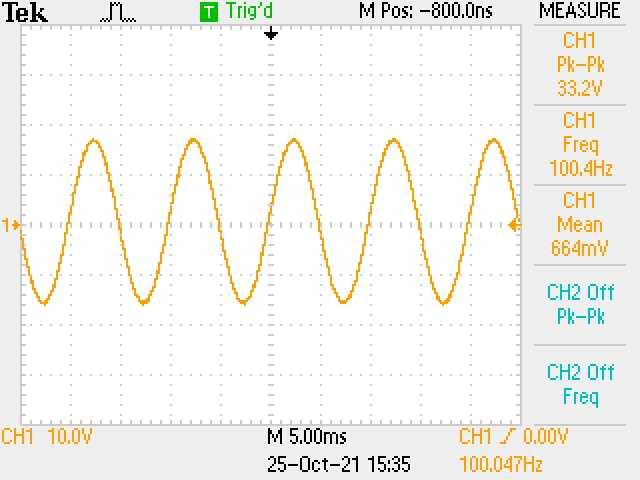
\includegraphics[width=\columnwidth]{power_output/filter_output_100Hz.JPG}
        \subcaption{100Hz}
        \label{F:out_100hz}
    \end{subfigure}
    \begin{subfigure}{0.3\textwidth}
        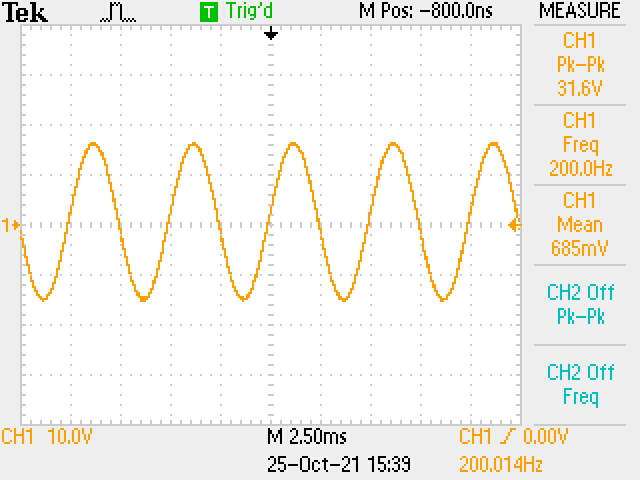
\includegraphics[width=\columnwidth]{power_output/filter_output_200Hz.JPG}
        \subcaption{200Hz}
        \label{F:out_200hz}
    \end{subfigure}
    \begin{subfigure}{0.3\textwidth}
        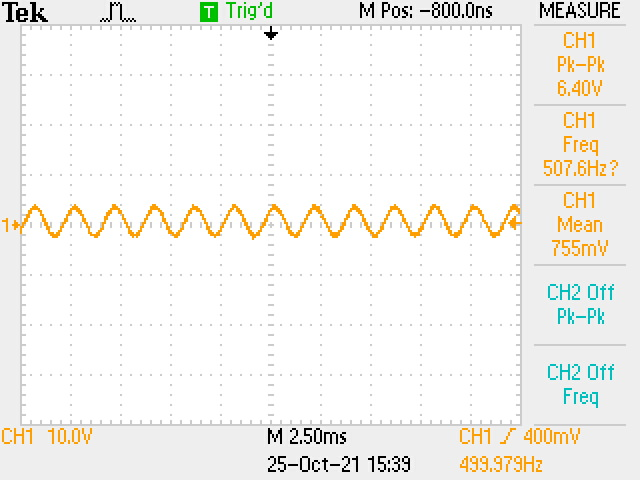
\includegraphics[width=\columnwidth]{power_output/filter_output_500Hz.JPG}
        \subcaption{500Hz}
        \label{F:out_500hz}
    \end{subfigure}
    \begin{subfigure}{0.3\textwidth}
        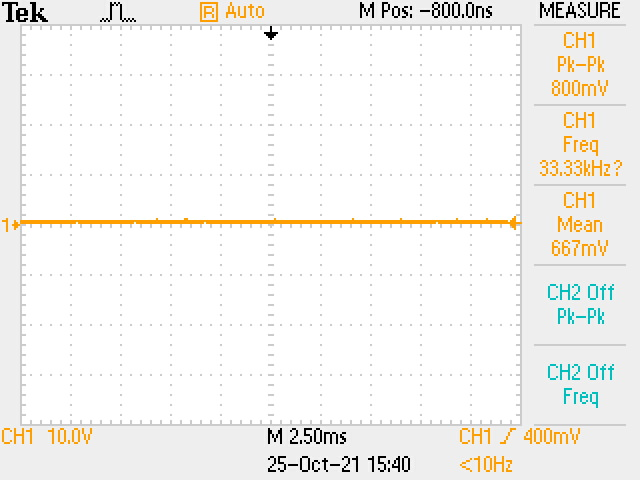
\includegraphics[width=\columnwidth]{power_output/filter_output_2kHz.JPG}
        \subcaption{2kHz}
        \label{F:out_2khz}
    \end{subfigure}
    \label{F:output_plotting}
    \caption{Amplifier output to varying frequency input signal}
\end{figure}

After observing the outputs waveforms, a bode plot was constructed through the use of the oscilloscope fast Fourier transform (FFT). The bode plot can be seen in \Cref{F:bode}, and it is exactly as expected.

\begin{figure}[H]
    \centering
    \frame{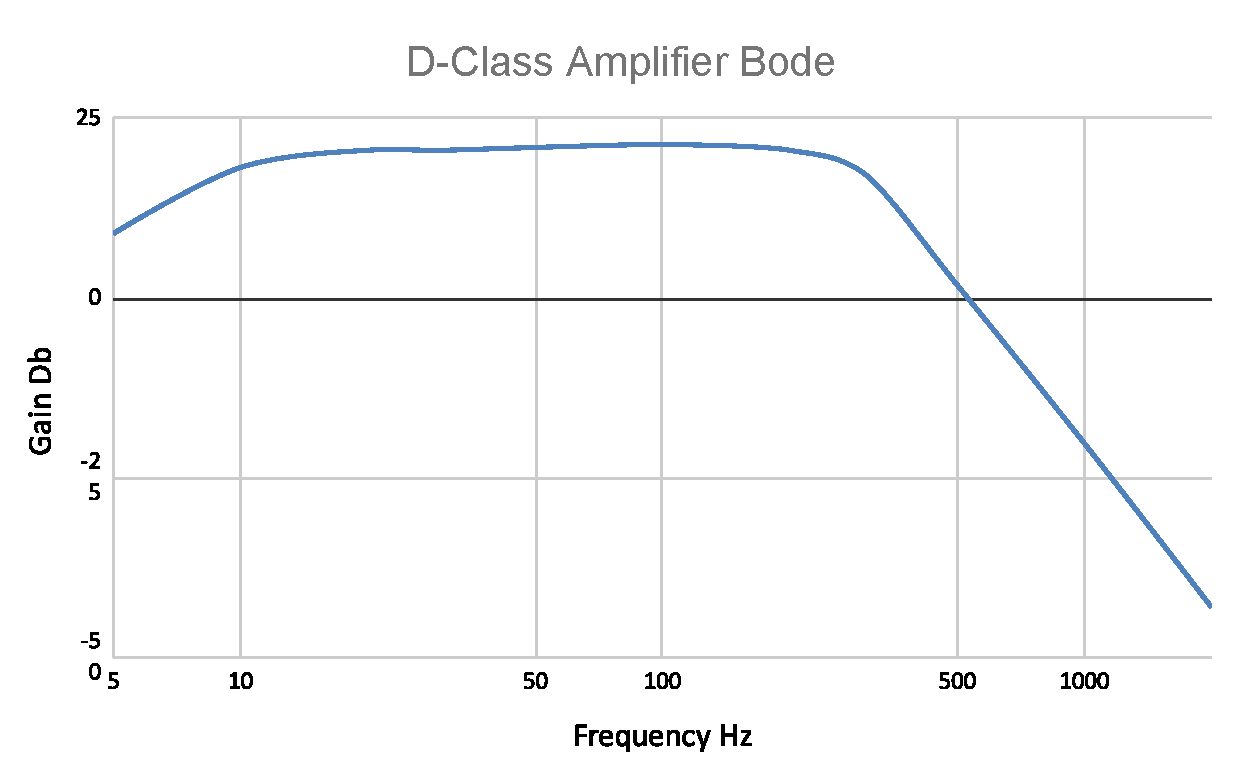
\includegraphics[width=0.85\textwidth]{power_output/amplifier_bode.pdf}}
    \caption{Amplifier output bode plot}
    \label{F:bode}
\end{figure}

Next, an efficiency plot of the amplifiers output was generated, plotting the output efficiency across the amplifiers frequency range, seen in \Cref{F:efficiency}. From this figure we can clearly see the the amplifiers efficiency is between 86\% and 92\% across the amplifiers bandwidth, with the efficiency greatly decreasing as soon as the filters are attenuating the output signal.

\begin{figure}[h!]
    \centering
    \frame{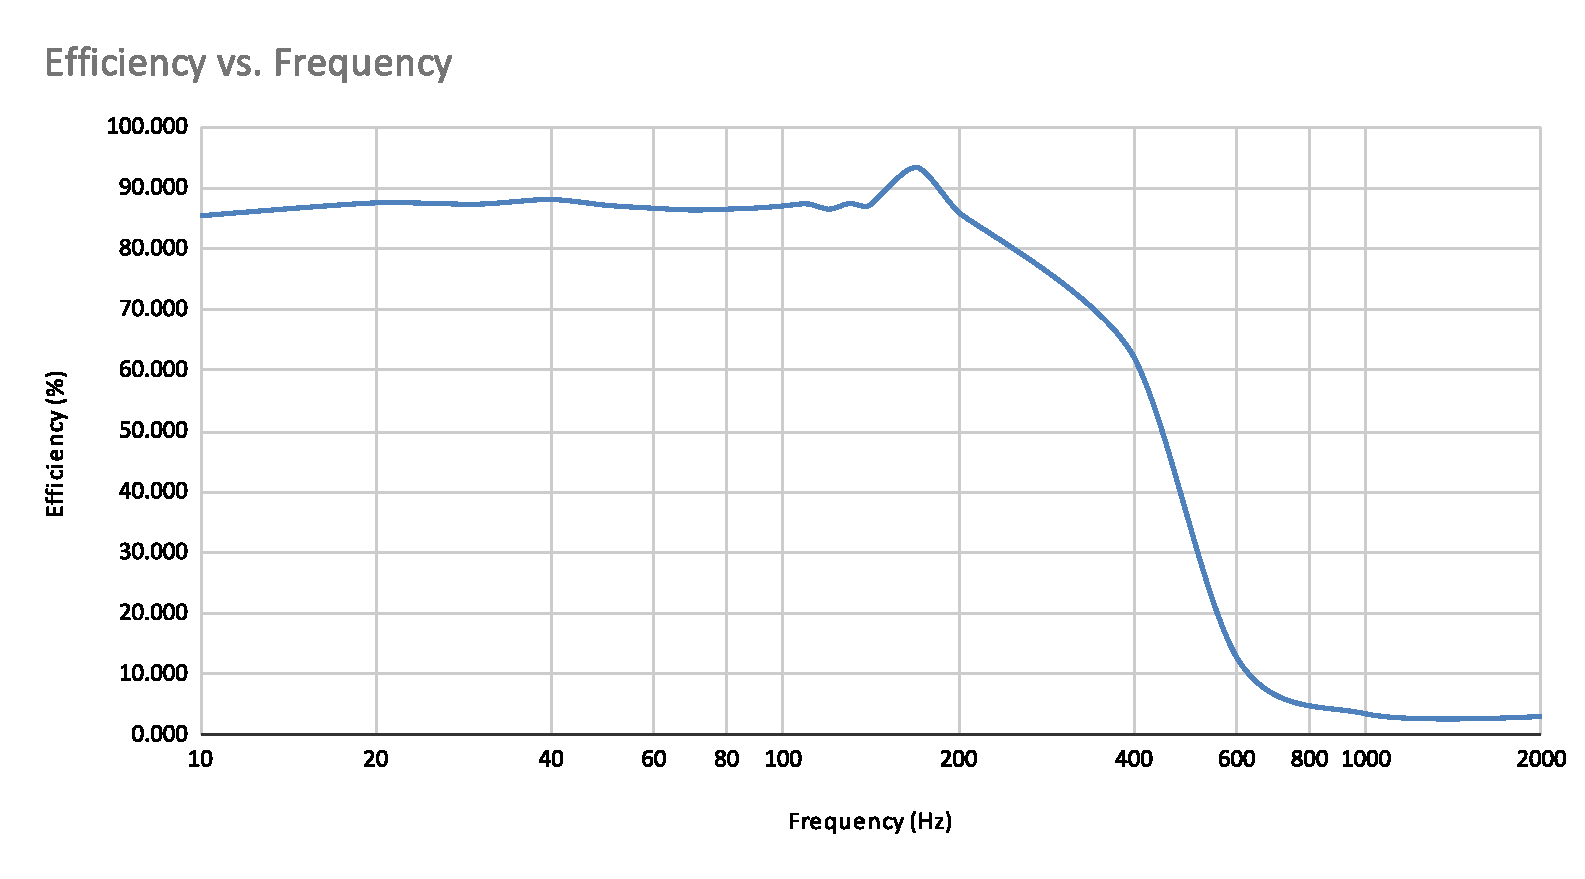
\includegraphics[width=0.85\textwidth]{power_output/Efficiency_vs._Frequency.pdf}}
    \caption{Amplifier output efficiency vs frequency}
    \label{F:efficiency}
\end{figure}

The final measurements taken of the amplifier were its total harmonic distortion across its frequency range. This can be seen in \Cref{T:THD}.

\begin{table}[h!]
    \centering
    \begin{tabular}{|l|l|}
    \rowcolor[HTML]{E0E0E0} 
    \textbf{Frequency (Hz)} & \textbf{THD (\%)} \\ \hline
    30                 & 1.8               \\
    50                 & 2.2               \\
    100                & 3.2               \\
    200                & 3.3               \\
    300                & 3.5               \\
    500                & 3.2              
    \end{tabular}
    \caption{Output total harmonic distortion across frequency}
    \label{T:THD}
\end{table}

\section{Conclusions}

Overall, our design and implementation of a class D amplifier was highly successful. We were able to achieve all of the specified requirements outlined in \Cref{S:specs}, while also keeping the \href{https://niels-clayton.github.io/D-Class_Amplifier/}{bill of materials (BOM)} for each amplifier to under \$50. This has allowed us to each build our own amplifier that we have been able to take home. The output waveform is undistorted and correctly attenuates all unwanted frequencies, while providing a high efficiency high power audio output.\\

All designed sections functioned as intended, and all minor changes to the design have been updated within the project to reflect those additions.\\

In conclusion, I believe that \Cref{F:lab_gang} successfully summarises the result of this project.

\begin{figure}[h!]
    \centering
    \frame{
\includegraphics[width=0.85\textwidth]{Danny_B.jpg}}
    \caption{Me and the ECEN lab crew listening to my class D amplifier OBLITERATE some pop song}
    \label{F:lab_gang}
\end{figure}


\clearpage
\section*{Appendix}
\subsection*{Input Filter}
\begin{figure}[h!]
  \centering
  \begin{subfigure}{0.3\textwidth}
    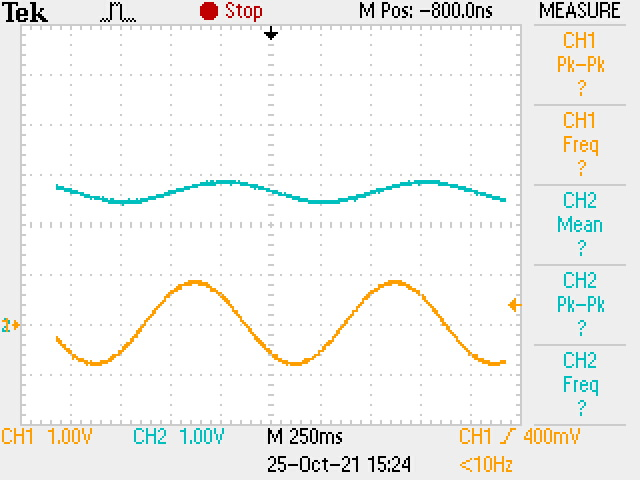
\includegraphics[width=\columnwidth]{input_filter/input_1Hz.JPG}
    \subcaption{1Hz}
  \end{subfigure}
  \begin{subfigure}{0.3\textwidth}
    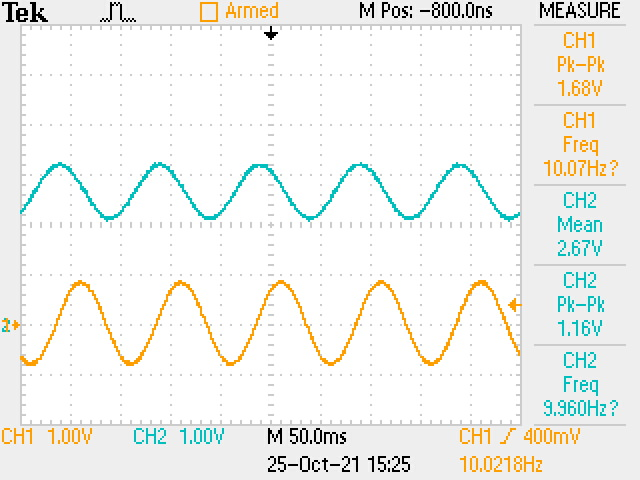
\includegraphics[width=\columnwidth]{input_filter/input_10Hz.JPG}
    \subcaption{10Hz}
  \end{subfigure}
  \begin{subfigure}{0.3\textwidth}
    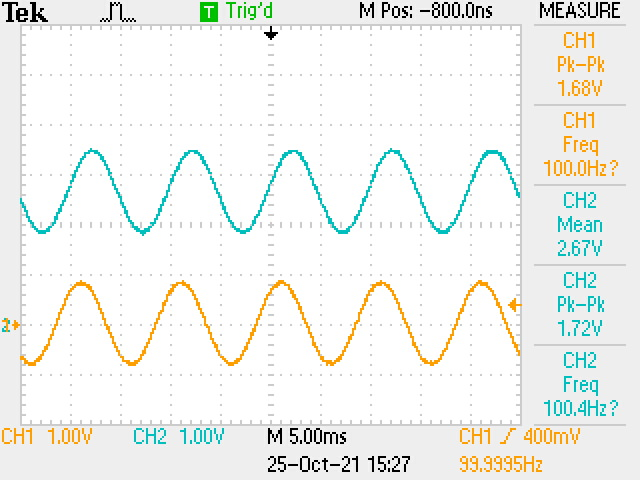
\includegraphics[width=\columnwidth]{input_filter/input_100Hz.JPG}
    \subcaption{100Hz}
  \end{subfigure}
  \begin{subfigure}{0.3\textwidth}
    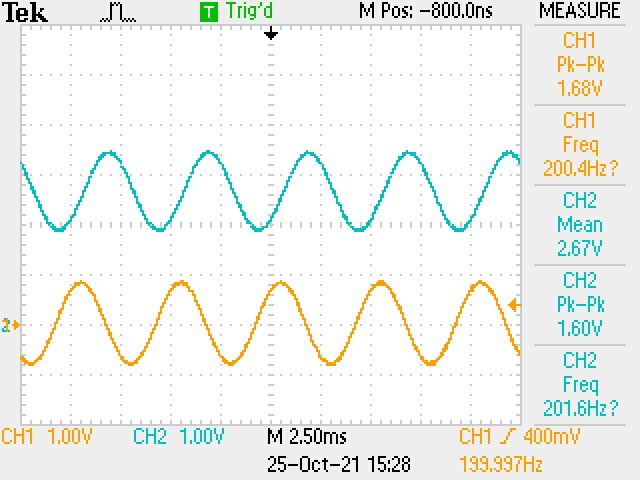
\includegraphics[width=\columnwidth]{input_filter/input_200Hz.JPG}
    \subcaption{200Hz}
  \end{subfigure}
  \begin{subfigure}{0.3\textwidth}
    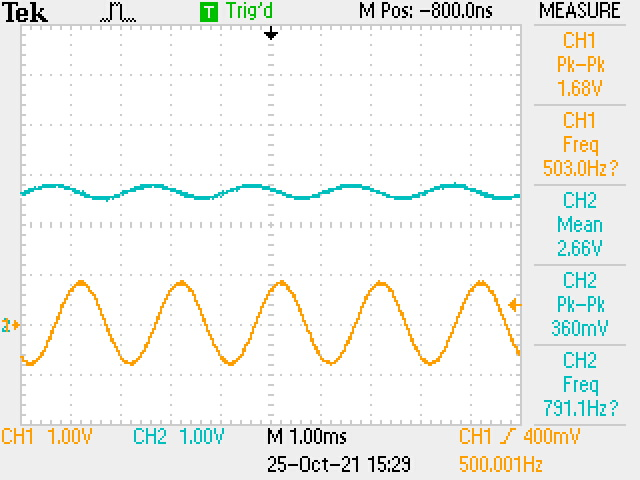
\includegraphics[width=\columnwidth]{input_filter/input_500Hz.JPG}
    \subcaption{500Hz}
  \end{subfigure}
  \begin{subfigure}{0.3\textwidth}
    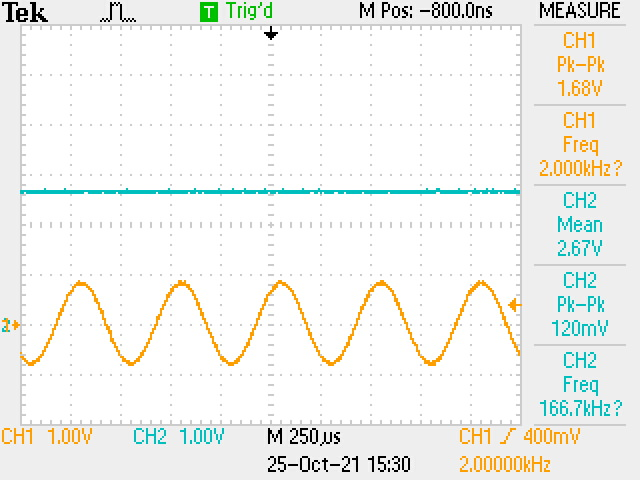
\includegraphics[width=\columnwidth]{input_filter/input_2kHz.JPG}
    \subcaption{2kHz}
  \end{subfigure}
  \caption{Input filter operation across frequencies, input signal (yellow) vs filter output (blue)}
\end{figure}


\end{document}